\documentclass{article}
\usepackage{graphicx} 
\usepackage{amsmath}
\usepackage{gauss, amssymb}
\usepackage{nicematrix}
\usepackage[utf8]{inputenc}
\usepackage[T1]{fontenc}
\usepackage[english]{babel}
\usepackage[nottoc,notlot,notlof]{tocbibind}
\usepackage[hidelinks]{hyperref}
\usepackage{amsthm}
\usepackage{physics}
\usepackage{booktabs}
\usepackage{nicematrix}
\usepackage{tikz}
\usepackage{pgfplots}
\usepackage{geometry}
\usepackage{tcolorbox}
\pgfplotsset{compat=1.18}

\theoremstyle{definition}
\newtheorem{definition}{Definition}[section]


\newcommand{\mycomment}[1]{}

% Define \circled
\newcommand*\circled[1]{\tikz[baseline=(char.base)]{
            \node[shape=circle,draw,inner sep=1pt] (char) {#1};}}

\title{5730.26 Tráðleyst samskifti V26 \\ Notes}
\date{}
%This material is based upon the book 
\begin{document}

\maketitle

\tableofcontents

\newpage

\section{Signal and Noise}


\subsection{Material reference}
Content from TSE Book

\begin{itemize}
    \item Chapter 1 (Sections 1.1 and 1.2): overview of wireless communication
    \item Appendix A.1: Gaussian random variables
    \item Appendix A.2 (look through): signal detection in Gaussian noise
\end{itemize}


\noindent
Content from Haykin

\begin{itemize}
    \item Chapter 2.2 (page 8 to 14) 
    \item Chapter 2.8 (page 47 to 55)
\end{itemize}

\subsection{Fundamental Quantities and Signal Representation}

In wireless communication systems, voltage and power are closely related but conceptually distinct quantities. Voltage is an electrical potential difference measured in volts, while power represents the rate of energy transfer and is measured in watts. In resistive systems, power is proportional to the square of voltage, which is why power-based metrics dominate wireless analysis. Because received signal strengths can vary across many orders of magnitude, logarithmic units are used almost exclusively.

Wireless systems typically operate at high frequencies, ranging from kilohertz in legacy systems to gigahertz and beyond in modern cellular and satellite communications. High-frequency signals enable higher data rates and smaller antennas, but they are also more susceptible to attenuation, noise, and hardware imperfections. As frequency increases, the impact of thermal noise and propagation loss becomes more pronounced, making signal-to-noise ratio a central performance metric.

A received signal is always corrupted by noise, which is any unwanted disturbance that alters the signal. In most wireless systems, thermal noise dominates and is well modeled as additive white Gaussian noise. This noise is statistically independent of the transmitted signal and has a power that depends on temperature and bandwidth.

\subsection{Power in dBm and Logarithmic Representation}

Absolute power in wireless systems is often expressed in decibels relative to one milliwatt, denoted as dBm. The conversion from linear power to dBm is given by
\[
P_{\mathrm{dBm}} = 10 \log_{10}\left(\frac{P}{1\,\mathrm{mW}}\right).
\]
This logarithmic representation allows convenient comparison of power levels and simplifies link budget calculations. Power gains and losses, such as antenna gain or path loss, are expressed in decibels (dB), which represent ratios rather than absolute values.

A power gain expressed in decibels is defined as
\[
G_{\mathrm{dB}} = 10 \log_{10}\left(\frac{P_{\text{out}}}{P_{\text{in}}}\right),
\]
while absolute power is expressed in dBm. This distinction is important: dB values can be added and subtracted freely, while dBm represents an actual physical power level.

\section{Logarithmic Identities}

Logarithmic manipulation is fundamental in wireless communication analysis. For base-10 logarithms, the identities
\[
\log_{10}(ab) = \log_{10}(a) + \log_{10}(b), \quad
\log_{10}\left(\frac{a}{b}\right) = \log_{10}(a) - \log_{10}(b),
\]
and
\[
\log_{10}(a^n) = n \log_{10}(a)
\]
are used extensively when converting between linear and logarithmic domains. For base-2 logarithms, which arise naturally in information theory, the same identities hold with $\log_2$ replacing $\log_{10}$. Base-2 logarithms are particularly important when expressing data rates in bits per second.

\section{Signal Composition and Noise Model}

A signal in the time domain may be composed of multiple frequency components. For example,
\[
x(t) = 2\sin(t) + \sin(5t)
\]
represents the superposition of two sinusoidal signals with different amplitudes and frequencies. Such decompositions are fundamental to Fourier analysis and spectral interpretation.

In a noisy channel, the received signal is modeled as
\[
y(t) = x(t) + n(t),
\]
where $n(t)$ is additive noise. This model underpins most digital communication theory and allows performance analysis in terms of probability of error and signal-to-noise ratio.

\subsection{Filters and Frequency Selectivity}

Filters are used to control which frequency components of a signal are passed or attenuated. A low-pass filter allows frequencies below a cutoff frequency to pass, while attenuating higher frequencies. A high-pass filter does the opposite, passing high frequencies and suppressing low frequencies. Band-pass filters pass only a specific range of frequencies, while notch (band-stop) filters suppress a narrow frequency band while allowing others to pass.

\subsubsection{Filter Visualizations}

\begin{figure}[h]
\centering
\begin{tikzpicture}
\begin{axis}[
    width=10cm,
    height=5cm,
    xlabel={Frequency},
    ylabel={Magnitude},
    ymin=0, ymax=1.1,
    domain=0:10,
    samples=200,
    axis lines=left
]
\addplot[thick] {1/(1 + exp(3*(x-4)))};
\end{axis}
\end{tikzpicture}
\caption{Low-pass filter magnitude response}
\end{figure}

\begin{figure}[h]
\centering
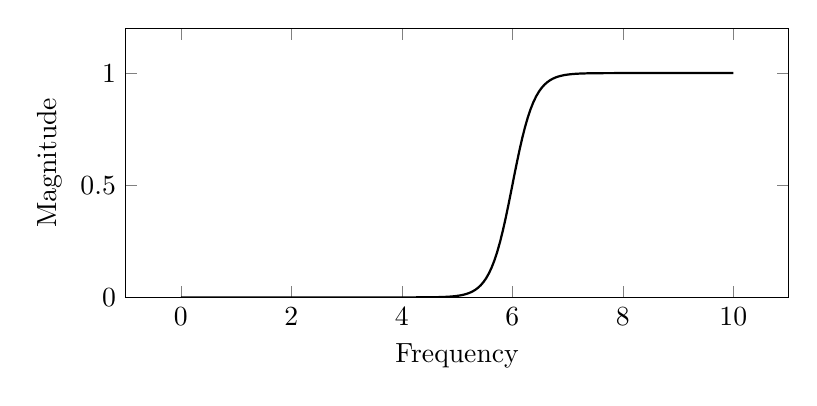
\begin{tikzpicture}
\begin{axis}[
    width=10cm,
    height=5cm,
    xlabel={Frequency},
    ylabel={Magnitude},
    ymin=0, ymax=1.2,
    domain=0:10,
    samples=200
]
\addplot[thick] {1/(1+exp(-5*(x-6)))}; 
\end{axis}
\end{tikzpicture}
\caption{High-pass filter magnitude response}
\end{figure}

\subsection{Link Budget and Measurement Instruments}

A link budget accounts for all gains and losses between the transmitter and receiver. The received power is given by
\[
P_{\mathrm{rx}} = P_{\mathrm{tx}} + G_{\mathrm{tx}} + G_{\mathrm{rx}} - L_{\mathrm{path}} - L_{\mathrm{other}},
\]
where all quantities are expressed in dB or dBm as appropriate. This equation provides an intuitive way to assess whether a communication link will close under given conditions.

Measurements are typically performed using a spectrum analyzer to observe signal power as a function of frequency, or a vector network analyzer to characterize frequency-dependent behavior such as gain, phase, and reflection. During lectures, readings in the range of 47–51 dBm were observed, indicating strong received signals or high reference levels depending on instrument configuration.

\subsection{Noise, Temperature, and Bandwidth}

Thermal noise power depends on temperature and bandwidth and is given in linear form by
\[
P_n = k_B T B,
\]
where $k_B$ is Boltzmann’s constant, $T$ is the absolute temperature in kelvin, and $B$ is the bandwidth in hertz. In logarithmic units, the noise power spectral density at room temperature is approximately $-174$ dBm/Hz. The total noise power in bandwidth $B$ is
\[
P_n = -174 + 10\log_{10}(B),
\]
with $B$ expressed in hertz.

Increasing bandwidth increases noise power but allows higher data rates. Narrow bandwidths provide finer spectral detail, while wider bandwidths are often easier to interpret and support higher throughput.

\subsection{Shannon Capacity and Energy Efficiency}

The maximum achievable data rate of a communication channel is given by Shannon’s capacity formula
\[
C = B \log_2(1 + \gamma),
\]
where $\gamma = \frac{P_s}{P_n}$ is the signal-to-noise ratio. This expression highlights diminishing returns: capacity grows logarithmically with SNR, meaning large power increases yield relatively small data rate improvements.

Energy efficiency is often expressed in bits per joule, or equivalently bits per watt-second. Communication systems are fundamentally limited by available power, and increasing spectral efficiency often comes at the cost of higher energy consumption.

\subsection{Modulation, BER, and Performance Metrics}

Information may be conveyed through amplitude, frequency, or phase modulation. Voice systems historically relied on analog modulation, while modern data systems use digital modulation schemes such as phase-shift keying. For PSK modulation, performance is often characterized using the ratio $E_b/N_0$, which relates the energy per bit to the noise spectral density.

The bit error rate (BER) quantifies the probability that a transmitted bit is incorrectly received. If $E = x - y$ denotes the error between transmitted and received bits, then the mean of $E$ corresponds to the BER. Experimental observations often show that distributions at power levels such as $-6$ dBm overlap significantly, indicating similar error behavior under those conditions.

\begin{figure}[h]
\centering
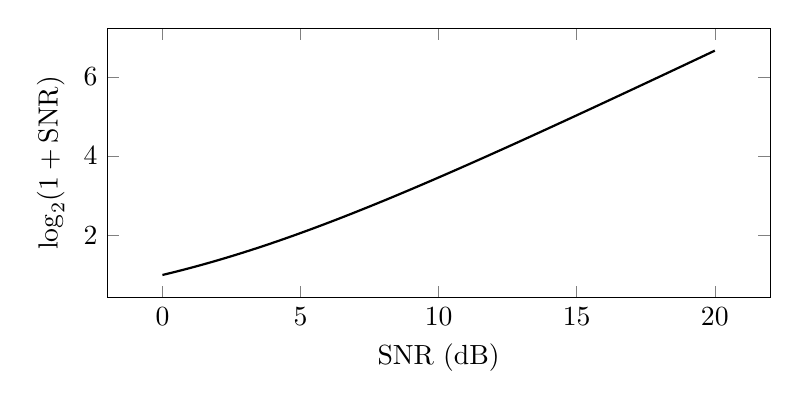
\begin{tikzpicture}
\begin{axis}[
    width=10cm,
    height=5cm,
    xlabel={SNR (dB)},
    ylabel={$\log_2(1+\mathrm{SNR})$},
    domain=0:20,
    samples=200
]
\addplot[thick] {ln(1 + 10^(x/10))/ln(2)};
\end{axis}
\end{tikzpicture}
\caption{Logarithmic growth of capacity with SNR}
\end{figure}



\newpage
%====================================================
\section{Lecture 2}

\subsection{Modulation}

In practical wireless systems, information cannot be transmitted directly at baseband over long distances. Antennas are physically inefficient at very low frequencies, and multiple users cannot share the spectrum effectively without frequency separation. 

For this reason, a baseband message signal $m(t)$ is shifted to a higher frequency using a carrier wave of frequency $f_c$. This process is known as modulation.

The simplest modulation process multiplies the baseband signal by a cosine carrier:

\[
s(t) = m(t)\cos(2\pi f_c t).
\]

Here, $f_c$ is called the carrier frequency, and it determines where the transmitted signal appears in the frequency spectrum.

Modulation therefore performs two key roles:
\begin{enumerate}
    \item Enables practical radiation through antennas.
    \item Allows multiple signals to coexist at different carrier frequencies.
\end{enumerate}

%====================================================
\subsection{Baseband and Bandpass Signals}

A baseband signal is centered around 0 Hz in the frequency domain. Its spectrum extends from $-B$ to $B$, where $B$ is the bandwidth of the signal.

After modulation, the signal becomes a bandpass signal whose spectrum is centered at $f_c$.

\subsubsection*{Baseband Spectrum}

\begin{center}
\begin{tikzpicture}
\draw[->] (-4,0) -- (4,0) node[right] {Frequency};
\draw[->] (0,0) -- (0,2);
\draw[thick] (-1.5,0) -- (-1.5,1.5);
\draw[thick] (1.5,0) -- (1.5,1.5);
\node at (0,-0.6) {0 Hz};
\node at (0,-1.2) {Baseband};
\end{tikzpicture}
\end{center}

\subsubsection*{Bandpass Spectrum}

\begin{center}
\begin{tikzpicture}
\draw[->] (0,0) -- (10,0) node[right] {Frequency};
\draw[->] (0,0) -- (0,2);
\draw[thick] (3,0) -- (3,1.5);
\draw[thick] (7,0) -- (7,1.5);
\node at (5,-0.6) {$f_c$};
\node at (5,-1.2) {Bandpass};
\end{tikzpicture}
\end{center}

The bandwidth of the bandpass signal remains:

\[
B = f_H - f_L.
\]

A fundamental efficiency metric is spectral efficiency:

\[
\eta = \frac{R_b}{B}.
\]

This measures how efficiently bandwidth is used to transmit information.

%====================================================
\subsection{Amplitude Modulation (AM)}

In amplitude modulation, the amplitude of the carrier is varied proportionally to the message signal:

\[
s(t) = A_c [1 + k_a m(t)] \cos(2\pi f_c t).
\]

The quantity $k_a$ controls how strongly the message influences the carrier amplitude.

The modulation index is:

\[
\mu = k_a \max |m(t)|.
\]

If $\mu > 1$, the envelope crosses zero, causing overmodulation and distortion.

AM is simple to implement but inefficient in power because a large portion of transmitted energy resides in the carrier.

\subsubsection*{AM Envelope}

\begin{center}
\begin{tikzpicture}[scale=1]
\draw[->] (-0.5,0) -- (6,0) node[right] {$t$};
\draw[->] (0,-2) -- (0,2);
\draw[domain=0:6,smooth,variable=\x,blue]
plot ({\x},{(1+0.5*sin(2*pi*\x/4))*sin(2*pi*\x)});
\draw[domain=0:6,smooth,variable=\x,red,dashed]
plot ({\x},{(1+0.5*sin(2*pi*\x/4))});
\draw[domain=0:6,smooth,variable=\x,red,dashed]
plot ({\x},{-(1+0.5*sin(2*pi*\x/4))});
\end{tikzpicture}
\end{center}

%====================================================
\subsection{Double Sideband Suppressed Carrier (DSB-SC)}

If the carrier is removed and only the product $m(t)\cos(2\pi f_c t)$ is transmitted, the scheme is called DSB-SC.

\[
s(t) = m(t)\cos(2\pi f_c t).
\]

The resulting spectrum consists of two shifted copies of the baseband spectrum, producing bandwidth:

\[
B_{DSB} = 2B.
\]

This improves power efficiency but still occupies twice the baseband bandwidth.

%====================================================
\subsection{Frequency Modulation (FM)}

In frequency modulation, information is conveyed by varying the instantaneous frequency of the carrier:

\[
s(t) = A_c \cos\left(2\pi f_c t + 2\pi k_f \int m(t) dt \right).
\]

The peak frequency deviation is:

\[
\Delta f = k_f A_m.
\]

Unlike AM, FM has constant amplitude, making it more resistant to noise.

Practical bandwidth is estimated using Carson’s rule:

\[
B_{FM} = 2(\Delta f + B).
\]

This shows that FM bandwidth increases with deviation.

%====================================================
\subsection{Phase Modulation (PM)}

In phase modulation, the carrier phase varies directly with the message:

\[
s(t) = A_c \cos(2\pi f_c t + k_p m(t)).
\]

FM and PM are closely related. Both belong to the class of angle modulation schemes.

%====================================================
\subsection{Complex Baseband Representation}

Bandpass signals can be expressed using complex notation:

\[
s(t) = I(t) + jQ(t) = A e^{j\theta}.
\]

This representation simplifies analysis and forms the foundation of digital modulation techniques.

Symbols are transmitted over finite intervals:

\[
R_s = \frac{1}{T_s}.
\]

If $M$ symbols are used:

\[
R_b = R_s \log_2 M.
\]

Higher $M$ increases data rate but reduces noise tolerance.

%====================================================
\subsection{Multipath Propagation}

Wireless signals rarely follow a single direct path. Instead, reflections from buildings, ground, and objects create multiple delayed copies of the signal.

This leads to:
\begin{itemize}
\item Inter-Symbol Interference (ISI)
\item Fading
\end{itemize}

\begin{center}
\begin{tikzpicture}
\node (tx) at (0,0) {Tx};
\node (rx) at (8,0) {Rx};
\draw[->] (tx) -- (rx);
\draw[->] (tx) to[out=40,in=140] (rx);
\draw[->] (tx) to[out=-40,in=-140] (rx);
\end{tikzpicture}
\end{center}

%====================================================
\subsection{Free Space Propagation Model (Exam Important)}

In ideal free space:

\[
P_r = P_t \left(\frac{\lambda}{4\pi d}\right)^2.
\]

Since $\lambda = \frac{c}{f_c}$, higher carrier frequencies produce greater path loss.

Received power decays proportionally to:

\[
d^2.
\]

This quadratic decay is fundamental in link budget design.

%====================================================
\subsection{Duplexing}

Communication may occur in one or both directions:

Simplex allows one-way communication.

Half-duplex allows two-way communication, but not simultaneously.

Full-duplex allows simultaneous transmission and reception.

%====================================================
\subsection{Multiple Access Techniques}

To allow multiple users to share limited spectrum, several strategies are used.

FDMA separates users in frequency.

TDMA separates users in time.

CDMA separates users using orthogonal codes:

\[
s(t) = m(t)c(t).
\]

Modern systems use OFDM and OFDMA to dynamically allocate subcarriers.

%====================================================
\subsection{Path Loss Model}

Real environments are more complex than free space. A general empirical model is:

\[
PL(d) = PL(d_0) + 10n \log_{10}\left(\frac{d}{d_0}\right).
\]

The exponent $n$ depends on the environment.

%====================================================
\subsection{Channel Behavior}

Wireless channels may be:
Line-of-sight (LOS), where a direct path exists.
Time-invariant, where channel conditions remain stable.
Time-variant, where motion causes fading and Doppler effects.
Understanding channel behavior is essential for robust system design.

%\newpage
%\section{Regression}

Regression analysis is a fundamental statistical technique used to model and understand the relationship between a response variable \( Y \) and one or more explanatory variables \( X_1, X_2, \ldots, X_p \). The goal is to estimate a function \( f(X) \) that captures the systematic relationship between \( X \) and \( Y \), while accounting for random variation (error).

\subsection{Additive Error Models}

We often assume an additive model of the form:
\[
Y = f(X) + \varepsilon,
\]
where \( \varepsilon \) is a random error term with
\[
\mathbb{E}[\varepsilon] = 0, \quad \text{and} \quad \text{Var}(\varepsilon) = \sigma^2.
\]
The term \( \varepsilon \) captures the \textbf{irreducible error}—random variation that cannot be explained by the model, even with perfect knowledge of \( f \).

A common goal is to estimate the \textbf{regression function}:
\[
f(X) = \mathbb{E}[Y|X].
\]
This represents the expected value of \( Y \) for a given value of \( X \).

\subsection{Estimating \( f(X) \)}

Given a set of training data \((x_1, y_1), \ldots, (x_n, y_n)\), we want to construct an estimate \(\hat{f}(X)\) that minimizes the expected prediction error:
\[
\mathbb{E}\left[(Y - \hat{f}(X))^2\right].
\]

\subsubsection{K-Nearest Neighbour (KNN) Regression}

A simple non-parametric estimator is the \textbf{K-nearest neighbours (KNN)} regression:
\[
\hat{f}(x_0) = \frac{1}{K} \sum_{x_i \in \mathcal{N}_K(x_0)} y_i,
\]
where \(\mathcal{N}_K(x_0)\) is the set of the \(K\) closest training points to \(x_0\).

\paragraph{Example:}
For example, to predict \( f(4) \), we take the average of the \(Y_i\) values for the \(K\) data points whose \(X_i\) values are closest to \(4\):
\[
\hat{f}(4) = \text{avg}\{Y_i : X_i \in \mathcal{N}_K(4)\}.
\]

\paragraph{Advantages and Limitations:}
\begin{itemize}
    \item Performs well when the number of predictors \(p\) is small and sample size \(n\) is large.
    \item Performs poorly when \(p\) is large due to the \textbf{curse of dimensionality}—as \(p\) increases, points become sparse, and distances between them lose meaning.
\end{itemize}

\begin{center}
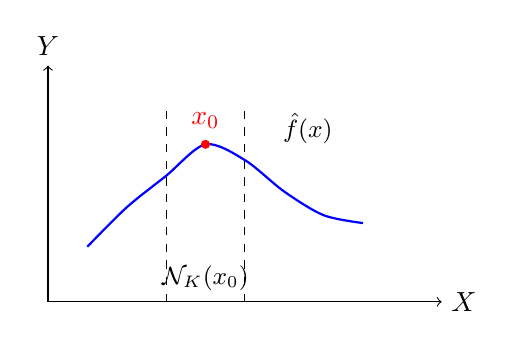
\begin{tikzpicture}[scale=1.0]
\draw[->] (0,0) -- (5,0) node[right] {$X$};
\draw[->] (0,0) -- (0,3) node[above] {$Y$};
\draw[blue, thick] plot[smooth] coordinates {(0.5,0.7) (1,1.2) (1.5,1.6) (2,2) (2.5,1.8) (3,1.4) (3.5,1.1) (4,1)};
\node at (3.3,2.2) {\small $\hat{f}(x)$};
\draw[red, fill=red] (2,2) circle (0.05);
\node[red] at (2,2.3) {$x_0$};
\draw[dashed] (1.5,0) -- (1.5,2.5);
\draw[dashed] (2.5,0) -- (2.5,2.5);
\node at (2,0.3) {\small $\mathcal{N}_K(x_0)$};
\end{tikzpicture}

\textit{Figure: KNN regression—averaging points within a neighbourhood around \(x_0\).}
\end{center}

\subsection{Parametric Models and Linear Regression}

To overcome the limitations of non-parametric methods like KNN, we often use a \textbf{parametric model} that assumes a specific functional form for \( f(X) \):
\[
f(X) = \beta_0 + \beta_1 X_1 + \beta_2 X_2 + \dots + \beta_p X_p.
\]

Even though this form is rarely exactly true, it provides a simple and interpretable approximation.

\subsubsection{Simple Linear Regression}

For a single predictor variable:
\[
Y = \beta_0 + \beta_1 X + \varepsilon.
\]

The goal is to estimate \( \beta_0 \) and \( \beta_1 \) using the training data, such that the \textbf{residual sum of squares (RSS)} is minimized:
\[
\text{RSS} = \sum_{i=1}^{n} (y_i - \hat{y}_i)^2 = \sum_{i=1}^{n} (y_i - \hat{\beta}_0 - \hat{\beta}_1 x_i)^2.
\]

Setting the partial derivatives of RSS with respect to \(\beta_0\) and \(\beta_1\) equal to zero yields the least-squares estimates.

\paragraph{Population Regression Line Example:}
\[
Y = 2 + 3X + \varepsilon \quad \Rightarrow \quad f(X) = 2 + 3X.
\]
Here, \(\beta_0 = 2\) and \(\beta_1 = 3\) are unbiased estimates of the true relationship between \(X\) and \(Y\).

\subsubsection{Standard Errors and Confidence Intervals}

The variance of the error term is denoted \(\sigma^2 = \text{Var}(\varepsilon)\).  
The estimated variance from data is:
\[
\widehat{\sigma}^2 = \frac{\text{RSS}}{n - 2}.
\]

The \textbf{standard error} of \(\hat{\beta}_1\) measures the uncertainty of the slope estimate.

A 95\% confidence interval for \(\beta_1\) is:
\[
[\hat{\beta}_1 - 2 \cdot SE(\hat{\beta}_1), \; \hat{\beta}_1 + 2 \cdot SE(\hat{\beta}_1)].
\]

\subsection{Hypothesis Testing}

We often test whether there is a significant relationship between \(X\) and \(Y\).

\[
\begin{aligned}
H_0 &: \beta_1 = 0 \quad \text{(no relationship)} \\
H_a &: \beta_1 \neq 0 \quad \text{(some relationship)}
\end{aligned}
\]

The test statistic is:
\[
t = \frac{\hat{\beta}_1 - 0}{SE(\hat{\beta}_1)},
\]
which follows a \(t\)-distribution with \(n - 2\) degrees of freedom under \(H_0\).

The \textbf{p-value} is the probability of observing a \( |t| \) as large as the one obtained, assuming \(H_0\) is true.  
A small p-value (typically \(< 0.05\)) leads to rejection of \(H_0\).

\subsection{Assessing Model Accuracy}

\subsubsection{Residual Standard Error (RSE)}

The RSE provides an estimate of the standard deviation of the residuals:
\[
RSE = \sqrt{\frac{RSS}{n - 2}}.
\]

\subsubsection{The \(R^2\) Statistic}

The \(R^2\) statistic measures the proportion of variability in \(Y\) explained by the model:
\[
R^2 = 1 - \frac{RSS}{TSS},
\]
where
\[
TSS = \sum_{i=1}^{n} (y_i - \bar{y})^2.
\]
Here, \(TSS\) measures the total variance in \(Y\), and \(RSS\) measures the remaining variability after regression.

\paragraph{Properties:}
\begin{itemize}
    \item \(R^2\) typically lies between 0 and 1.
    \item It can be negative for models that fit worse than a horizontal line at \(\bar{y}\).
    \item \(R^2\) is independent of the units of \(Y\).
\end{itemize}

\subsection{Bias–Variance Tradeoff}

When fitting regression models, we balance two sources of error:
\[
\text{Expected Test Error} = \text{Bias}^2 + \text{Variance} + \text{Irreducible Error}.
\]
Parametric models typically have higher bias but lower variance, while non-parametric models like KNN have lower bias but higher variance.

\subsection{Software Note: R and Quarto}

When working with R in VSCode, you can compile regression analyses and visualizations within \texttt{.qmd} (Quarto) files, which support both code and markdown text for reproducible reports.


%\newpage
%\section{Classification}

Classification problems involve predicting a qualitative (categorical) response variable \(Y\) based on one or more predictor variables \(X\).  

\subsection{Quantitative vs. Qualitative Outcomes}

\begin{itemize}
    \item \textbf{Quantitative outcomes:} \(Y \in \mathbb{R}\). Typically modeled with regression, minimizing a loss function such as least squares.
    \item \textbf{Qualitative outcomes:} \(Y \in \{1, 2, \dots, K\}\). These are modeled using classification methods like logistic regression or generative models.
\end{itemize}

\subsection{Feature Vector and Notation}

Let 
\[
\mathbf{X} = (X_1, X_2, \dots, X_p)^T
\] 
be the feature vector. For example, in the \textbf{IRIS dataset}, the features are:
\[
X_1 = \text{Sepal Length}, \quad X_2 = \text{Sepal Width}, \quad X_3 = \text{Petal Length}, \quad X_4 = \text{Petal Width}
\] 
and the response \(Y \in \{\text{setosa, versicolor, virginica}\}\).

The predicted class is:
\[
g(\mathbf{x}) = \arg\max_{k} P(Y = k \mid \mathbf{X} = \mathbf{x})
\]

\subsection{Logistic Regression (Binary Case)}

The probability of class 1 is modeled as:
\[
P(Y=1 \mid X=x) = \frac{e^{\beta_0 + \beta_1 x}}{1 + e^{\beta_0 + \beta_1 x}}
\]

The log-odds (logit) transformation gives a linear relationship:
\[
\log \frac{P(x)}{1 - P(x)} = \beta_0 + \beta_1 x
\]

\[
\begin{cases} 
\beta_1 > 0 & \text{increasing $x$ increases $P(x)$} \\
\beta_1 < 0 & \text{increasing $x$ decreases $P(x)$} 
\end{cases}
\]

\subsection{Maximum Likelihood Estimation (MLE)}

The likelihood function is:
\[
L(\beta_0, \beta_1) = \prod_{i=1}^{n} P(x_i)^{y_i} \left[ 1 - P(x_i) \right]^{1 - y_i}
\]

MLE maximizes the likelihood (or equivalently, minimizes the negative log-likelihood):
\[
\hat{\beta}_0, \hat{\beta}_1 = \arg\max_{\beta_0, \beta_1} L(\beta_0, \beta_1)
\]

\subsection{Multinomial Logistic Regression}

For \(K>2\) classes, probabilities are modeled using the \textbf{softmax function}:
\[
P(Y=k \mid X=x) = \frac{e^{\beta_{k0} + \beta_k^T x}}{\sum_{j=1}^{K} e^{\beta_{j0} + \beta_j^T x}}
\]

The log-odds relative to a baseline class \(K\) are:
\[
\log \frac{P(Y=k \mid X=x)}{P(Y=K \mid X=x)} = \beta_{k0} + \beta_k^T x
\]

\subsection{Generative Models}

Generative models estimate:
\[
P(X \mid Y=k) \quad \text{and} \quad P(Y=k)
\] 
Then, using Bayes' theorem:
\[
P(Y=k \mid X=x) = \frac{P(X=x \mid Y=k) P(Y=k)}{\sum_{j=1}^K P(X=x \mid Y=j) P(Y=j)}
\]

\subsection{Additive Models and Least Squares}

For continuous responses:
\[
Y = f_\theta(X) + \epsilon, \quad \epsilon \sim N(0, \sigma^2)
\]

MLE reduces to minimizing the sum of squared errors (RSS):
\[
\hat{\theta} = \arg\min_\theta \sum_i \left( Y_i - f_\theta(X_i) \right)^2
\]

\subsection{Visualizing Logistic Regression Decision Boundary}

\begin{tikzpicture}[scale=1.0]
\draw[->] (0,0) -- (6,0) node[right] {$X$};
\draw[->] (0,0) -- (0,4) node[above] {$P(Y=1|X)$};
\draw[domain=0:5, smooth, variable=\x, blue, thick] plot ({\x}, {4/(1+exp(-1*(\x-2)))});
\draw[dashed] (2,0) -- (2,2) -- (0,2);
\node at (3.5,3.5) {Sigmoid curve};
\node at (2.5,0.3) {$x_0$};
\end{tikzpicture}

\subsection{Generative Models and Advanced Classification}

Generative models estimate the joint distribution \(P(X,Y)\) and then use Bayes' theorem to compute class probabilities:
\[
P(Y=k \mid X=x) = \frac{P(Y=k) P(X=x \mid Y=k)}{P(X=x)}
\]

Here:
\begin{itemize}
    \item \(P(Y=k)\) is the prior probability of class \(k\)
    \item \(P(X=x \mid Y=k)\) is the class-conditional density
    \item \(P(X=x) = \sum_{i=1}^K P(Y=i) P(X=x \mid Y=i)\) by the law of total probability
\end{itemize}

\subsubsection{Linear Discriminant Analysis (LDA)}

LDA assumes that:
\begin{itemize}
    \item Each class \(k\) has a Gaussian distribution with mean \(\mu_k\) and a **common covariance matrix** \(\Sigma\)
    \item The decision boundary is linear in \(x\)
\end{itemize}

The discriminant function is:
\[
\delta_k(x) = x^T \Sigma^{-1} \mu_k - \frac{1}{2} \mu_k^T \Sigma^{-1} \mu_k + \log \pi_k
\]
where \(\pi_k\) is the prior probability of class \(k\).  

The predicted class is:
\[
\hat{y} = \arg\max_k \delta_k(x)
\]

We estimate unknown parameters from the data:
\[
\hat{\mu}_k = \frac{1}{n_k} \sum_{i: y_i=k} x_i, \quad
\hat{\Sigma} = \frac{1}{n-K} \sum_{k=1}^K \sum_{i: y_i=k} (x_i - \hat{\mu}_k)(x_i - \hat{\mu}_k)^T
\]

\subsubsection*{Decision Boundary Visualization (2 Classes, 2 Features)}
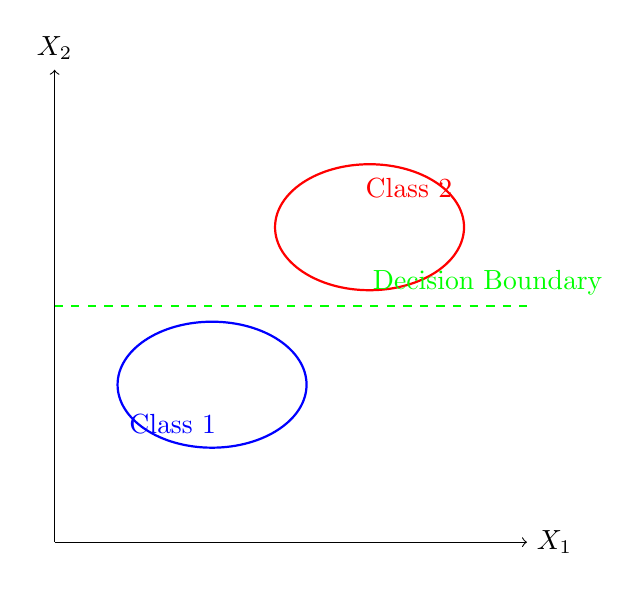
\begin{tikzpicture}[scale=1.0]
% axes
\draw[->] (0,0) -- (6,0) node[right] {$X_1$};
\draw[->] (0,0) -- (0,6) node[above] {$X_2$};

% class 1 ellipse
\draw[blue, thick] (2,2) ellipse (1.2cm and 0.8cm);
\node[blue] at (1.5,1.5) {Class 1};

% class 2 ellipse
\draw[red, thick] (4,4) ellipse (1.2cm and 0.8cm);
\node[red] at (4.5,4.5) {Class 2};

% linear decision boundary
\draw[green, thick, dashed] (0,3) -- (6,3);
\node[green] at (5.5,3.3) {Decision Boundary};
\end{tikzpicture}

\subsubsection{Quadratic Discriminant Analysis (QDA)}

QDA relaxes the LDA assumption of common covariance matrices:
\[
\Sigma_k \neq \Sigma_j \quad \text{for some } k \neq j
\]

The discriminant function becomes quadratic:
\[
\delta_k(x) = -\frac{1}{2} \log |\Sigma_k| - \frac{1}{2} (x - \mu_k)^T \Sigma_k^{-1} (x - \mu_k) + \log \pi_k
\]

\subsubsection{Naive Bayes Classifier}

Naive Bayes assumes that features are conditionally independent given the class:
\[
P(X_1, X_2, \dots, X_p \mid Y=k) = \prod_{j=1}^p P(X_j \mid Y=k)
\]

This allows simple estimation using Gaussian distributions for quantitative features or categorical probabilities for discrete features.

\subsubsection{K-Nearest Neighbors (KNN)}

\begin{itemize}
    \item Non-parametric and flexible
    \item Assigns a class based on the majority vote of the \(K\) nearest neighbors in feature space
    \item More data generally improves performance
\end{itemize}

\subsubsection{Bias-Variance Trade-off and Model Comparison}

\begin{itemize}
    \item LDA: Linear boundaries, low variance, higher bias
    \item QDA: Quadratic boundaries, higher variance, lower bias
    \item Logistic Regression: Linear boundary, sensitive to collinearity
    \item KNN: Highly flexible, low bias, potentially high variance
\end{itemize}

\subsubsection{Performance Metrics}

\begin{itemize}
    \item \textbf{Accuracy:} Overall correct classification
    \item \textbf{Sensitivity / Recall:} True positive rate
    \item \textbf{Specificity:} True negative rate
    \item \textbf{ROC curve:} Trade-off between sensitivity and false positive rate
\end{itemize}

\subsubsection{Other Notes}

\begin{itemize}
    \item Poisson regression for count data: \(n \sim \text{Poisson}(\mu)\) with \(\log(\mu) = X \beta\)
    \item More data allows more flexible models (e.g., QDA, KNN) to perform well without overfitting
\end{itemize}


\end{document}
